\section{Introduction}
\label{sec:intro}

The OpenMP effort began in 1996 with a handful of vendors (DEC, HP, IBM, Intel,
Kuck and Associates, and SGI) came together to create a portable application
programming interface~(API) for shared memory computers.  Vendors do not
typically work well together unless an outside force compels cooperation.  In
this case, that compulsion came from the parallel tools team working within the
Accelerated Strategic Computing Initiative~(ASCI) who made it clear that to sell
machines into the ASCI program, a vendor had to join the effort to create a
portable API for shared memory programming.  DOE researchers played a key role
in defining OpenMP from the beginning helping to assure that the API met the
needs of HPC applications programmers.

The goals of the initial group were spelled out in early public presentations
about the project~\cite{ewomp99}.
%The OpenMP Architecture Review Board and the future of OpenMP, Tim Mattson,
%European Workshop on OpenMP, Lund, Sweden, September 30 - October 1, 1999

\begin{itemize}
  \item To define an API that lets programmer write portable, efficient and well
    understood parallel programs for shared memory systems.
  \item To produce specifications based on common practice that could be readily implemented.
  \item To whatever extent makes sense, the API should be consistent between Fortran, C,
    and C++.
  \item OpenMP must remain lean and mean; being just large enough to express important
    control-parallel, shared memory programs  but no larger.
  \item Legal programs under older versions of the specification must continue to be legal
    under new specifications.
  \item To whatever extent possible, correct OpenMP programs should produce the same result
    when run as serial programs or as parallel programs.
\end{itemize}

The first OpenMP specification  was released in November 1997 at SC'97.   The
OpenMP community in the late 90's were painfully aware of other parallel
programming  standardization efforts such as HPF and MPI 2.0; both of which
suffered from multi-year delays as implementors struggled to produce robust,
application-ready implementations.  Hence, OpenMP by design was narrowly
focused on current practice and within a year of its initial release, multiple
vendor supported implementations were available.

Over time, additional vendors and research organizations joined the effort.  A
non-profit corporation, the OpenMP Architecture Review Board, was incorporated
to reduce the chances that any single vendor could inappropriately dominate the
standard.

As hardware capabilities and the need to support a wider range of algorithms
grew, the complexity of the specification expanded.  We can see this in
Figure~\ref{omppcount} where the pages of the specifications (not including
appendices or indices) are listed.   The initial OpenMP specification (OpenMP
Version 1.0 for Fortran) was around 45 pages long.  The  latest specification
(OpenMP 4.5 for Fortran, C and C++)  has over 300 pages.

We also see the evolution of language support in OpenMP in
Figure~\ref{omppcount}.  Prior to version 2.5 of the specification released in
2005, an OpenMP specification was specialized to a particular language.   This
made writing the text of the specification much easier, but given that most of
the people working on the Fortran specifications also worked on the C/C++
specifications, we could not run the two language committees in parallel.  This
led to long delays between updated specifications such as the almost 4 year
delay between OpenMP 1.0 for C/C++ and OpenMP 2.0 for C/C++.  The process of
merging the two languages into a single specification was a much larger
undertaking than any of us expected at the time and required us to go back and
recast the core abstractions behind OpenMP much more carefully so they would
apply across languages.  The resulting OpenMP version 2.5 specification took
three years to create.

OpenMP is no longer a simple API the full breadth of which can be learned in
less than a day.  Features were added to address non-uniform memory
architectures, more complex concurrency control, irregular algorithms,
accelerators, and much more.   Specification do not grow due to a lack of
discipline by the designers.  They grow as users demand new features and
hardware changes.  In that light, an almost seven-fold increase in size over the
course of almost 20 years is not surprising.

\begin{figure}
  \centering
  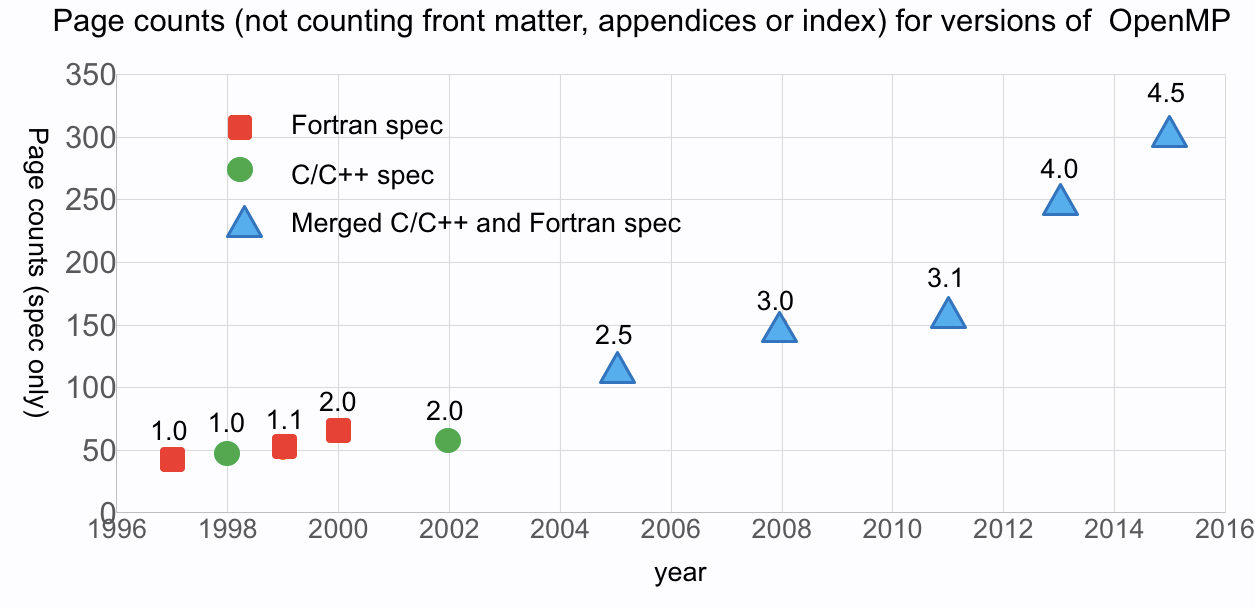
\includegraphics[width=3.4in]{pics/opcounts.png}
  \caption{OpenMP specification release dates, page counts and language bindings.}
  \label{omppcount}
\end{figure}


